\documentclass[10pt,a4paper]{article}
\usepackage{rpgcover} % Loads the original rpgmanual.sty and its fonts
\babelprovide[import]{spanish}
\usepackage{xsavebox}
\RPGSetRunningTitle{El sendero de las deudas}
\hypersetup{pdftitle={El sendero de las deudas — La última tirada},pdfauthor={Jacopo Biscella}}
\RPGSetCoverWordSpace{.78em}
% Paragraph spacing and leading of the Spanish adventure and manual-es.tex.
\setlength{\parskip}{3.85pt plus .5pt minus .5pt}
\linespread{1.115}\selectfont
% JPEG copies of the shared cover backgrounds (scripts/build-adventure-print-art.sh), as in the adventure.
\RPGSetFrontBackground{assets/engraved-front-background.jpg}\RPGSetBackBackground{assets/engraved-cover-background.jpg}
% The adventure's front-cover typography, with the overlay saved once (xsavebox) and reused on the
% contents page instead of being embedded twice.
\newcommand{\SentieroFrontCover}{%
 \clearpage\RPGCoverPagetrue\thispagestyle{empty}\null
 \xsavebox{SentieroOverlay}{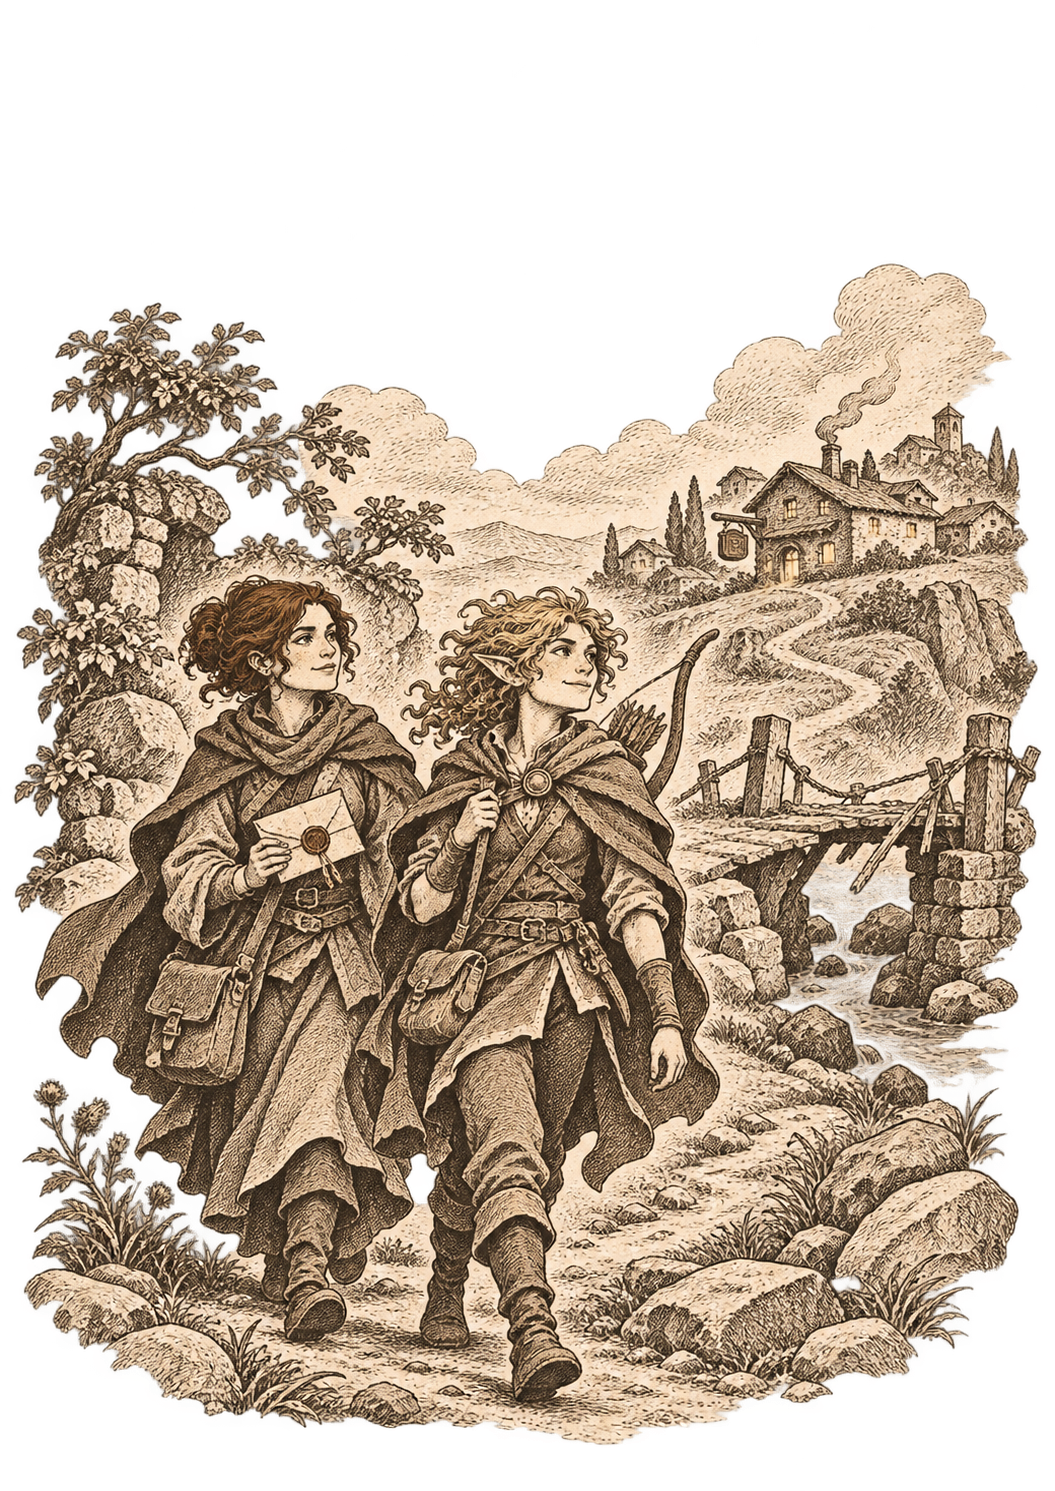
\includegraphics{assets/path-of-debts/front-overlay.png}}%
 \begin{tikzpicture}[remember picture,overlay,x=1mm,y=1mm]
  \RPGDrawBackground{\RPGFrontBackgroundFile}
  % Title and subtitle as on the adventure's cover: same sizes and positions in the cartouche.
  \node[align=center,text=coverink,text width=138mm,inner sep=0pt] at ($(current page.south west)+(105mm,248mm)$)
   {\RPGCoverTitleFont\fontsize{16.6}{20.7}\selectfont\spaceskip=\RPGCoverWordSpace\relax EL SENDERO\\[1.0mm]DE LAS DEUDAS};
  \node[align=center,text=coverink,text width=135mm,inner sep=0pt] at ($(current page.south west)+(105mm,235mm)$)
   {\RPGCoverSubtitleFont\fontsize{9.5}{12}\selectfont Un relato introductorio para «La última tirada»};
  \node[inner sep=0pt,anchor=center] at ($(current page.south west)+(105mm,125mm)$)
   {\resizebox{150mm}{!}{\xusebox{SentieroOverlay}}};
  \node[align=center,text=coverink,text width=124mm,inner sep=0pt] at ($(current page.south west)+(105mm,25mm)$)
   {\RPGCoverTextFont\fontsize{12}{15}\selectfont Jacopo Biscella};
 \end{tikzpicture}
 \clearpage\RPGCoverPagefalse}
% Uses precisely the back background and the editable cover fonts from rpgcover.sty.
% This is text layout only: no substitute illustrations or background graphics.
\newcommand{\SentieroBackCover}{%
 \clearpage\pagenumbering{gobble}\RPGCoverPagetrue\thispagestyle{empty}\null
 \begin{tikzpicture}[remember picture,overlay,x=1mm,y=1mm]
   \RPGDrawBackground{\RPGBackBackgroundFile}
   \node[align=center,text=coverink,text width=170mm,inner sep=0pt]
     at ($(current page.south west)+(105mm,260mm)$)
     {{\RPGCoverTitleFont\fontsize{19}{23}\selectfont\spaceskip=\RPGCoverWordSpace\relax EL SENDERO DE LAS DEUDAS}};
   \draw[coverink,line width=.45pt]
     ($(current page.south west)+(57mm,246mm)$)--($(current page.south west)+(153mm,246mm)$);
   % Blocks at the positions of the adventure's back cover: story at 240 mm, small-caps lines at
   % 197, second rule at 167, description at 162, closing line at 133.
   \node[anchor=north,align=left,text=coverink,text width=137mm,inner sep=0pt]
     at ($(current page.south west)+(105mm,240mm)$)
     {\RPGCoverTextFont\fontsize{10.4}{13.4}\selectfont
      Una moneda falsa. Una carta sin destinatario. Dos viajeros sin motivos para fiarse el uno del otro.\par\smallskip
      Nim Thistledown y Mara Veyne siguen el camino del rey hasta Hogar Hueco. Durante el viaje descubrirán que una promesa puede ser más peligrosa que un arma, y que algunas decisiones tienen consecuencias aunque nadie las vea.};
   \node[anchor=north,align=center,text=coverink,text width=140mm,inner sep=0pt]
     at ($(current page.south west)+(105mm,197mm)$)
     {\RPGCoverSubtitleFont\fontsize{13}{17}\selectfont
      Un prólogo a «La campana de Hogar Hueco»};
   \draw[coverink,line width=.45pt]
     ($(current page.south west)+(57mm,167mm)$)--($(current page.south west)+(153mm,167mm)$);
   \node[anchor=north,align=left,text=coverink,text width=137mm,inner sep=0pt]
     at ($(current page.south west)+(105mm,162mm)$)
     {\RPGCoverTextFont\fontsize{10.4}{13.4}\selectfont
      Siete ejemplos muestran cómo las decisiones de los jugadores se convierten en tiradas, diálogos y consecuencias en la mesa de La última tirada.};
   \node[anchor=north,align=center,text=coverink,text width=147mm,inner sep=0pt]
     at ($(current page.south west)+(105mm,133mm)$)
     {\RPGCoverSubtitleFont\fontsize{10.5}{13.2}\selectfont
      El relato termina donde empieza la aventura.};
   \filldraw[fill=white,draw=coverink,line width=.55pt]
     ($(current page.south west)+(139mm,25mm)$) rectangle
     ($(current page.south west)+(187mm,55mm)$);
 \end{tikzpicture}
 \clearpage\RPGCoverPagefalse
}
% Dice icons for the "En la mesa" boxes, drawn with TikZ (no font glyphs, so they work in every
% language). \Dado{n}: a kept d6 showing n; \Dado*{n}: a rolled die that is not kept (faded).
% \Su and \Giu: the rulebook's keep-highest and keep-lowest arrows, from FreeSerif.
% \Bersaglio: the TN to reach. \Riuscita and \Fallita: success and failure.
\newcommand\DadoPips[1]{%
  \ifcase#1\or \fill (.5,.5) circle (.1);
  \or \fill (.27,.73) circle (.1); \fill (.73,.27) circle (.1);
  \or \fill (.25,.75) circle (.09); \fill (.5,.5) circle (.09); \fill (.75,.25) circle (.09);
  \or \foreach \x/\y in {.27/.27,.27/.73,.73/.27,.73/.73}{\fill (\x,\y) circle (.095);}
  \or \foreach \x/\y in {.25/.25,.25/.75,.75/.25,.75/.75,.5/.5}{\fill (\x,\y) circle (.09);}
  \or \foreach \x/\y in {.28/.22,.28/.5,.28/.78,.72/.22,.72/.5,.72/.78}{\fill (\x,\y) circle (.085);}
  \fi}
\makeatletter
% A die that is set aside has a dashed outline and lighter pips, but stays legible.
\tikzset{dado kept/.style={draw=rpgbrown,fill=white},dado dropped/.style={draw=rpgbrown,fill=rpgshade,dash pattern=on .9pt off .6pt},
  pips kept/.style={fill=rpgink},pips dropped/.style={fill=rpgbrown!70}}
\newcommand\Dado{\@ifstar{\Dado@{dropped}}{\Dado@{kept}}}
\newcommand\Dado@[2]{\tikz[baseline=-.1em,x=.95em,y=.95em]{%
  \path[dado #1,line width=.5pt,rounded corners=1.2pt] (0,-.12) rectangle (1,.88);
  \begin{scope}[shift={(0,-.12)},pips #1]\DadoPips{#2}\end{scope}}}
\makeatother
\newcommand\Su{{\fontspec{FreeSerif}↑}}
\newcommand\Giu{{\fontspec{FreeSerif}↓}}
\newcommand\Riuscita{\tikz[baseline=-.1em,x=1em,y=1em]{\draw[rpgbrown,line width=1.1pt,line cap=round,line join=round] (.08,.35)--(.38,.05)--(.92,.75);}}
\newcommand\Fallita{\tikz[baseline=-.1em,x=1em,y=1em]{\draw[rpgbrown,line width=1.1pt,line cap=round] (.15,.05)--(.85,.75) (.15,.75)--(.85,.05);}}
\newcommand\Bersaglio{\tikz[baseline=-.1em,x=1em,y=1em]{\draw[rpgbrown,line width=.6pt] (.5,.38) circle (.45) (.5,.38) circle (.25); \fill[rpgbrown] (.5,.38) circle (.08);}}
\begin{document}
% Select the language here: babel resets to its main language (english) at \begin{document}.
\selectlanguage{spanish}
\RPGStartFrontMatter
\SentieroFrontCover
\RPGStartContents
\clearpage\thispagestyle{rpgfrontmatter}
\vspace*{9mm}
\begin{center}{\fontsize{27}{31}\selectfont\bfseries ÍNDICE\par}\vspace{9pt}
{\color{rpgline}\rule{.76\linewidth}{.55pt}}\end{center}\vspace{8mm}
\begingroup
\makeatletter
\renewcommand{\l@section}[2]{\@dottedtocline{1}{0em}{4em}{\bfseries #1}{#2}}
\@starttoc{toc}
\makeatother
\endgroup
\vfill
\begin{center}\resizebox{.58\linewidth}{!}{\xusebox{SentieroOverlay}}\end{center}
\vfill
\begin{center}{\small\itshape Un relato introductorio para La última tirada\par}
\vspace{4pt}{\footnotesize Jacopo Biscella\par}\vspace{5pt}
{\footnotesize Este relato se distribuye bajo Creative Commons Atribución–CompartirIgual 4.0 Internacional (CC BY-SA 4.0), en las mismas condiciones que La última tirada. Se permite compartir y adaptar el material, incluso comercialmente, citando al autor y manteniendo la licencia en las obras derivadas.\par}\end{center}
\clearpage
\RPGStartMainMatter
\RPGChapter{Una mala moneda}
La moneda tenía dos caras. Una llevaba la corona del rey; la otra, el rostro de un hombre al que el rey había mandado ahorcar veinte años atrás.

El erudito Mara Veyne la hizo girar entre el pulgar y el índice. El cobre estaba gastado por un solo lado. Quien la había acuñado quería que el engaño durase poco: lo bastante para cambiar de manos, no lo bastante para llegar a los ojos de un recaudador.

«Ya te he dicho que es falsa», dijo el mercader.

«No he dicho lo contrario».

«¿Entonces por qué llevas media hora mirándola?»

«Para averiguar quién quiere usarla».

Estaban sentados a una mesa de la casa de postas de Tres Vados. Llovía desde hacía cuatro días. El camino del rey se había convertido en una larga franja de barro por la que carros y caballos avanzaban a duras penas. El mercader le había vendido a Mara un asiento en el carro para el tramo hacia el norte, junto con una promesa: podría consultar el libro de mercancías antes de llegar a la encrucijada.

Aquella promesa, Mara lo había comprendido, valía más que el viaje.

El libro enumeraba las aldeas que recorría el carro. Entre ellas, con otra letra, figuraba \textbf{Hogar Hueco}. Junto al nombre alguien había trazado una marca redonda y luego la había tachado.

«Ese sitio ya no está en mi ruta», dijo el mercader al ver adónde miraba.

«¿Desde cuándo?»

«Desde que el precio de la madera dejó de cubrir el coste del viaje».

«¿Y esa marca?»

El hombre cerró el libro. «Una tontería, para no perder la cuenta de una entrega. El carro sale al alba. ¿Todavía vienes?»

Mara dejó la moneda sobre la mesa, con el rey hacia arriba. «Sí».

No le contó al mercader que había visto una letra parecida años atrás, en el margen de un viejo registro. Tampoco le preguntó por qué alguien había raspado una fecha para escribir otra. Había aprendido que las preguntas hechas demasiado pronto vuelven prudentes incluso a los mentirosos más torpes.

Esa noche copió el nombre de la aldea al final de sus notas. Luego cambió de ruta. El carro iría al norte. Mara, en la encrucijada, tomaría el sendero del bosque.
\begin{rpgnote}
\textbf{Cómo leer los recuadros.} En los recuadros \emph{En la mesa} los dados aparecen dibujados: \Dado{5}~dado que se conserva, \Dado*{2}~dado descartado, \Bersaglio~NO que hay que alcanzar, \Riuscita~éxito, \Fallita~fallo. Los niveles se escriben como en la hoja: Inexperto 2d6\Giu\ (conserva el menor), Competente 1d6, Experto 2d6\Su\ (conserva el mayor), Excepcional 3d6\Su. El NO es el Número Objetivo, el valor que hay que alcanzar. Cerca es una de las distancias del manual: a pocos pasos, alcance inmediato.
\end{rpgnote}
\begin{rpgexample}{En la mesa · La primera tirada}
\textbf{Narrador:} «El mercader cierra el libro. Mara ha visto el nombre de la aldea y una fecha raspada. A primera vista la fecha es ilegible. ¿Cómo intentas descifrarla?»

\textbf{Jugador de Mara:} «Comparo el trazo de los números con las otras fechas de la misma mano. No uso Historia: no necesito recordar qué pasó, necesito leer marcas borradas».

\textbf{Narrador:} «Entonces es Saber, \Bersaglio\,NO~4. Mara es Experto: tira 2d6\Su, dos dados, y conserva el mayor».

\textbf{Jugador de Mara:} «Saco \Dado*{2}\,\Dado{5}: conservo 5». \Riuscita

\textbf{Narrador:} «Lo consigues. La fecha es de hace dos semanas, no de ayer. El nombre de la aldea, en cambio, ya lo conocías: eso nunca dependió de la tirada».

\emph{Se tira cuando el resultado es incierto. El nivel Experto tira 2d6 y conserva el mejor dado: un 5 alcanza el NO~4. Una pista esencial nunca se esconde tras una tirada.}

\end{rpgexample}
\RPGChapter{El tercer camino}
Nim Thistledown no cogió la bolsa enseguida.

El carretero la sostenía abierta, con cara de quien espera que le den las gracias. Dentro había seis monedas de plata y una hoja de papel doblada en cuatro.

«El pago acordado», dijo.

«Por el camino que los dos conocemos, quizá».

«Por una entrega».

«¿Y por qué no la llevas tú?»

El carretero señaló su carro, parado con una rueda rota delante del establo. «Porque me faltan un caballo, una rueda y las ganas de que me maten por una carta».

Nim desdobló el papel. No estaba sellado. Contenía dos líneas: \emph{La mitad de la deuda está pagada. La otra mitad, en plata del norte, cuando la campana calle.} Al pie figuraba el nombre de una posada de Hogar Hueco, pero no el de su destinatario.

«¿Quién te ha dado esto?»

«Un hombre en la encrucijada. Capa gris, capucha puesta. Decía las palabras correctas con el acento donde no tocaba, como quien las ha aprendido de oído».

Nim volvió a doblar la hoja. «¿Y su nombre?»

«No me lo dio. Me dio plata. ¿La coges o no?»

Nim cogió la bolsa, pero contó las monedas una a una. La sexta era fina, casi lisa. «Faltan dos».

El carretero suspiró y añadió una moneda. Nim se alejó antes de que pudiera cambiar de idea.

No tenía intención de entregar la carta a ciegas. Era dinero suficiente para tres días de camino; demasiado para un mensaje sin nombre. Y una campana que debía callar no era una frase para entregar sin entenderla.

El tercer camino empezaba detrás de los establos, donde el barro guardaba pocas huellas. Un sendero rápido, según el mapa; abandonado, según la gente del lugar. Nim se puso en marcha contando los pasos hasta la primera bifurcación.
\RPGChapter{El árbol caído}
Mara encontró a Nim pasado el mediodía, ante un tronco que cerraba el sendero.

Nim estudiaba el suelo. Había dejado el morral sobre una piedra y sujetaba una ramita entre los dientes.

«¿Está cerrado el bosque?», preguntó Mara.

«Depende de lo que te gusten los atajos».

«No mucho».

«Entonces tenemos algo en común».

El tronco de un haya atravesaba el paso, con las raíces todavía hundidas en la tierra. Había caído hacía poco. Las hojas estaban verdes; la corteza, húmeda. No había soplado un viento lo bastante fuerte para derribarlo.

Mara se agachó a mirar una astilla. Del corte rezumaba savia clara.

«Un hacha», dijo.

«Dos», respondió Nim. «Una trabajó por este lado y otra por el otro».

Mara miró las muescas: paralelas, regulares, demasiado bajas para alguien que buscara leña. «Lo talaron solo para cerrar el sendero».

«Hay huellas que vuelven atrás. Al otro lado, ninguna».

«¿Sabes leer huellas?»

«Sé ver dónde alguien ha intentado borrarlas».

Mara sonrió apenas. Nim se deslizó bajo el tronco, salió con una manga embarrada y señaló un estrecho hueco entre las raíces. «Se puede pasar, pero quien lleve un carro tendrá que dar media vuelta».

«¿Y quien lleve libros?»

«Depende de cuántos».

Mara dio unas palmadas a su zurrón. «Demasiados».

No se dijeron sus nombres hasta haber dejado atrás el obstáculo. No era una gran prueba de confianza. Pero Mara dejó de llevarse la mano al cierre del zurrón cada vez que Nim se le acercaba.
\RPGChapter{El desprendimiento}
Encontraron el desprendimiento casi una hora después.

El sendero corría a media ladera, por encima de un arroyo crecido. Durante unos veinte pasos desaparecía: la lluvia había arrancado una franja de la pendiente, y en su lugar bajaba hasta el agua una lengua de barro y piedras. De vez en cuando una piedra se soltaba y rodaba ladera abajo sin prisa. Alguien había pasado el día anterior: las huellas llegaban hasta la mitad y se perdían bajo un corrimiento más reciente.

Nim estudió la ladera. «Podríamos volver a subir hasta el vado».

«¿Cuánto tardaríamos?»

«Dos horas, quizá tres».

Mara alzó la vista. Las nubes habían vuelto a tapar el sol. «¿Y cuánto falta para la aldea?»

«Otra media jornada».

«Entonces llegaríamos de noche».

Nim miró el desprendimiento. Donde el barro había dejado la roca al descubierto, un pie podía encontrar apoyo; en otros puntos la tierra cedía en cuanto se la tocaba. «Si cruzo rápido y ligera, la ladera no tendrá tiempo de moverse».

«También podrías caerte».

«Es una de las posibilidades».

Mara se ajustó la correa del zurrón sobre el pecho. «Entonces no cruzas sola. Iré detrás de ti, pondré los pies donde los pongas tú y te sujetaré por el cinturón. Si resbalas, te sostendré».

«Y si resbalas tú, me arrastrarás contigo».

«Pues procura no hacerme resbalar».

Nim lo miró un momento. Luego se volvió hacia el desprendimiento y echó a andar. Mara la siguió, con una mano bien agarrada a su cinturón.

A mitad de camino, un terrón cedió bajo el pie de Nim. El barro se movió de golpe, como una manta de la que tiran por un lado. Nim se fue hacia delante; Mara afianzó los talones en una piedra y tiró. El cinturón aguantó. Durante un instante se quedaron quietos, mientras las piedras sueltas rodaban hasta el arroyo.

Después Nim encontró la roca, y Mara la siguió paso a paso.

Cuando llegaron al otro lado, a Mara le temblaban las piernas. Nim se volvió: el paso ya había desaparecido bajo una capa nueva de barro.

«Dos horas ahorradas», dijo.

«No has contado los diez años de vida que acabo de perder».

«Esos no venían en el mapa».
\begin{rpgexample}{En la mesa · Cruzar y ayudar}
\textbf{Narrador:} «El desprendimiento sigue moviéndose. Cruzarlo es Destreza, \Bersaglio\,NO~4. Si fallas, resbalas hacia el arroyo».

\textbf{Jugadora de Nim:} «Nim es Experta en Destreza: 2d6\Su. ¿Puede ayudarme Mara?»

\textbf{Jugador de Mara:} «Camino justo detrás de ella y la sujeto por el cinturón. Si resbala, la sostengo».

\textbf{Narrador:} «Cruzáis juntos y tira quien va delante: Nim. Mara es Inexperto en Destreza y no tiene ninguna Habilidad que le sirva: en la misma prueba no tiraría con nivel Experto, así que su ayuda es una ayuda incompetente. Añade un dado a la tirada de Nim, pero el NO sube de 4 a 5: dos personas sobre el barro sueltan más piedras. ¿Lo aceptáis?»

\textbf{Jugadora de Nim:} «Sí. Si resbalo sola, no tengo nada a lo que agarrarme».

\textbf{Narrador:} «Entonces Nim tira 3d6\Su\ contra \Bersaglio\,NO~5».

\textbf{Jugadora de Nim:} «Saco \Dado*{1}\,\Dado*{4}\,\Dado{5}: conservo 5». \Riuscita

\textbf{Narrador:} «Habéis cruzado. A mitad de camino un terrón cede bajo Nim, y Mara la sostiene por el cinturón. Al otro lado os dais la vuelta: el paso ya ha desaparecido bajo el barro. Por aquí no pasará ningún carro».

\emph{La ayuda incompetente añade 1d6, pero sube el NO en 1. Con 1, 4 y 5, Nim alcanza el nuevo NO~5. La mano de Mara en el cinturón es la forma en que la ayuda entra en la historia: no sustituye a la tirada.}

\end{rpgexample}
\RPGChapter{Dos personas en el camino}
Caminaron hasta que el sendero se hizo tan ancho como un camino. Entonces vieron el carro.

Tenía ruedas altas, la caja cubierta con un hule y un caballo gris que comía las hojas más bajas de un avellano. El conductor dormía en el pescante, con el sombrero sobre la cara. Una mujer estaba inclinada sobre el cubo de la rueda derecha.

«¿Podemos ayudar?», preguntó Mara.

La mujer se enderezó. Tenía las manos negras de grasa y un cuchillo de trabajo colgado del cinturón. «Si tenéis un pasador de repuesto».

Nim miró la rueda. «No hace falta cambiarlo. El seguro está doblado».

«¿Y tú cómo lo sabes?»

«Porque el pasador sigue en su sitio».

La mujer le tendió el martillo sin decir nada. Nim se agachó, hizo palanca con una piedra plana y dio tres golpes precisos. El seguro quedó casi recto.

«Prueba ahora», dijo.

La mujer tiró de la rueda. Giraba.

El conductor se despertó con el ruido. Preguntó quiénes eran, por qué tocaban el carro y si intentaban robarle. La mujer le dijo que se callara.

«¿Vais a Hogar Hueco?», preguntó Mara.

La mujer dejó de limpiarse las manos. «Pasábamos por allí, hasta hace poco».

«¿Y ahora?»

«Ahora preferimos perder un día».

No quiso decir más, pero les dio un pedazo de pan y un queso duro envuelto en una hoja. Cuando el conductor se distrajo, habló en voz baja.

«El camino del norte está lleno de hombres que cobran peajes sin tener derecho. No llevan uniforme. Uno de ellos lo llevó, en otro tiempo».

«¿Dónde?», preguntó Nim.

«En la encrucijada de las Tres Piedras. Si os lo encontráis, no digáis que me habéis ayudado».

Mara no insistió. Antes de reemprender la marcha, Nim se agachó junto a las rodadas. Entre las huellas del caballo había otras, de dos personas a pie: habían seguido el carro casi hasta el avellano y luego habían vuelto hacia el norte.

«No es un aviso de oídas», le dijo Nim a la mujer. «Ya os los habéis encontrado».

La mujer miró las huellas y asintió. «Uno es joven. El otro no se deja ver si puede evitarlo».

Los despidió con un gesto y volvió al carro.
\begin{rpgexample}{En la mesa · Cuando una Habilidad cambia la tirada}
\textbf{Narrador:} «El seguro está doblado. Nim, ¿cómo intentas arreglarlo?»

\textbf{Jugadora de Nim:} «Con el martillo de la mujer del carro y una piedra para apoyarlo».

\textbf{Narrador:} «Una reparación de verdad sería Saber con Artesanía. Aquí, en cambio, solo tienes que enderezar el seguro con tres golpes precisos: Destreza, \Bersaglio\,NO~4. Si fallas, puedes partirlo».

\textbf{Jugadora de Nim:} «Nim es Experta en Destreza: 2d6\Su. Ninguna de sus Habilidades tiene que ver con martillos, así que no sube ningún grado. Saco \Dado*{3}\,\Dado{5}: conservo 5». \Riuscita

\textbf{Narrador:} «La rueda vuelve a girar. Al poneros en marcha, ves huellas junto a las rodadas. ¿Quieres examinarlas?»

\textbf{Jugadora de Nim:} «Sí. Nim tiene Supervivencia, una Habilidad de Destreza que sirve justo para rastrear».

\textbf{Narrador:} «Averiguar quién siguió el carro es \Bersaglio\,NO~4. Destreza Experto más Supervivencia: subes un grado, a Excepcional. Tira 3d6\Su».

\textbf{Jugadora de Nim:} «Saco \Dado*{2}\,\Dado*{4}\,\Dado{6}: conservo 6». \Riuscita

\textbf{Narrador:} «Distingues dos rastros: siguieron el carro y luego giraron hacia el norte. La mujer confirma que ya se ha encontrado con los falsos recaudadores».

\emph{Los valores son los de la hoja de Nim: Experta en Destreza, con Supervivencia y sin Artesanía, que además es una Habilidad de Saber. Una Habilidad pertinente mejora la tirada un grado. Un solo 6 no es un Crítico: hacen falta al menos dos.}

\end{rpgexample}
\RPGChapter{La encrucijada de las Tres Piedras}
En la encrucijada había tres mojones, pero solo dos seguían en pie. El tercero yacía de costado, medio oculto en la hierba. Alguien había grabado una marca reciente en el musgo: un círculo atravesado por una línea.

Nim la reconoció como la marca de un recaudador ambulante. La había visto en recibos auténticos y falsos, más a menudo falsos que auténticos.

«El peaje es un timo», dijo.

«No es ninguna sorpresa».

«El sitio que han elegido, sí. Aquí no hay nada que valga la pena proteger».

«Un camino», respondió Mara, «es útil aunque no tenga nada alrededor».

Siguió un breve silencio. Luego llegó una voz desde detrás de los arbustos.

«Veinte monedas por pasar».

El hombre que salió al descubierto era joven. Llevaba una casaca que le quedaba grande, una lanza con la punta oxidada y dos botas desparejadas. Un segundo hombre se quedó entre los árboles, donde el sendero volvía a estrecharse.

«¿Veinte?», repitió Nim. «El rey debe de haberse vuelto generoso con sus recaudadores».

«No he dicho que sea del rey».

«Cierto. El rey habría tenido al menos el sentido común de mandar a alguien con un recibo».

El joven bajó la lanza hacia el pecho de Nim. Mara dio un paso adelante.

«Espera», le dijo al joven. «¿Quién os ha ordenado estar aquí?»

«Paga o da media vuelta».

«Si nos dejas pasar», continuó Mara, «no tendrás problemas. Si alguien te ha mandado a cobrar, también te habrá dicho adónde llevar el dinero».

El joven vaciló. El hombre escondido tosió.

Nim se giró de golpe y miró más allá de ellos. «Hay alguien en el camino».

El joven recaudador siguió su mirada un instante. Bastó. Nim empujó la punta de la lanza hacia abajo y pasó a su lado. Mara la siguió sin correr.

Desde los árboles llegó una maldición. Nadie los siguió.

Caminaron en silencio cien pasos; luego Mara dijo: «No había nadie detrás de nosotros».

«No he dicho que lo hubiera».

«Has dicho que había alguien en el camino».

«No. He dicho: “Hay alguien en el camino”. Nosotros estábamos en el camino».

Mara negó con la cabeza. No se reía, pero saltaba a la vista que tenía ganas.
\begin{rpgnote}[fontupper=\normalfont]\textbf{Joven recaudador} \emph{NO Fue3/Des3 · Competente · 2 Heridas · lanza (2H) · sin armadura.} \emph{Comportamiento: «Obedece órdenes, pero no quiere matar a nadie».}\end{rpgnote}
\begin{rpgexample}{En la mesa · Una tirada enfrentada}
\textbf{Narrador:} «El joven de la lanza os cierra el paso. El otro hombre espera entre los árboles. ¿Qué hacéis?»

\textbf{Jugadora de Nim:} «Finjo ver a alguien detrás de ellos, para distraerlos».

\textbf{Narrador:} «El joven te mira con recelo: es una tirada enfrentada de Saber, y no hay ningún NO que alcanzar. Nim es Inexperta en Saber y no tiene Engaño: tira 2d6\Giu\ y conserva el menor. El joven es Competente: 1d6».

\textbf{Jugadora de Nim:} «Saco \Dado{5}\,\Dado*{6}: conservo 5».

\textbf{Narrador:} «El joven saca \Dado{2}. Tu 5 es más alto: se da la vuelta y baja la lanza un momento. Podéis pasar a su lado mientras Mara lo entretiene hablando». \Riuscita

\textbf{Jugador de Mara:} «Le digo que nos deje ir: no quiero hacerle daño».

\emph{En una tirada enfrentada tiran las dos partes y gana el resultado más alto; un empate es un punto muerto. No hay un NO fijo. La tirada abre una oportunidad; no decide por sí sola todo lo que pasa después.}

\end{rpgexample}
\RPGChapter{El granero}
Volvió a llover poco antes del atardecer. Los dos viajeros se refugiaron en un granero abandonado, a doscientos pasos del camino. Una pared se había derrumbado; el tejado, en cambio, aguantaba.

Nim reunió una brazada de paja seca y la empujó contra la pared. Mara dejó sus libros sobre una caja vacía. Del fondo del granero llegaba un olor a lana mojada.

No estaban solos.

Detrás del pesebre había una niña sentada, envuelta en una manta que le quedaba grande. Tenía el pelo pegado a la frente y se aferraba a un saco de harina. A su lado dormía un perro flaco.

«No queremos tu saco», dijo Mara.

«No es mío».

«¿De quién es?»

La niña no contestó. Nim se sentó en el otro extremo del granero y se puso a limpiar el cuchillo con un trapo. Lo hizo de modo que la hoja nunca apuntara hacia la niña.

«¿Tienes nombre?», preguntó Mara.

«Tessa».

«¿Adónde vas, Tessa?»

«A casa de mi tío».

«¿Dónde vive?»

«Más adelante».

No necesitaban saber más para ver que tenía miedo. Mara abrió el pan que les había dado la mujer del carro y partió un trozo. Lo dejó sobre la caja, entre ellos.

Tessa esperó a que Mara volviera a su manta y luego cogió el pan.

Más tarde, cuando el perro se despertó, la niña les habló de unos hombres que habían llegado de noche a su casa, al otro lado del valle, para llevarse el grano. Su madre la había enviado a casa de su tío con el último saco de harina. La lluvia la había sorprendido a mitad de camino.

«Por la mañana podemos acompañarte hasta la próxima bifurcación», dijo Mara.

Nim no dijo nada. A la mañana siguiente, sin embargo, fue la primera en levantarse.
\begin{rpgexample}{En la mesa · Rasgo y Carga}
\textbf{Narrador:} «La niña no quiere hablar y aprieta el saco. ¿Qué hacéis?»

\textbf{Jugador de Mara:} «Le doy algo de comer y le dejo tiempo. No quiero interrogarla».

\textbf{Narrador:} «No hace falta tirar: el pan no compra su confianza, pero le demuestra que no sois una amenaza inmediata. Mara, ¿hay algo en tu Rasgo o en tu Carga que haga que esta decisión le importe?»

\textbf{Jugador de Mara:} «Sí. La Carga de Mara es una promesa que no puede cumplir. Me gustaría que Tessa se la recordara».

\textbf{Narrador:} «Entonces no te pido que la cuentes entera ahora. Esta noche, Mara se queda despierto más de lo necesario para asegurarse de que Tessa está a salvo».

\textbf{Jugadora de Nim:} «Podría preguntarle a la niña quién entró en su casa, pero no lo hago. Quiero que confíe en nosotros al menos lo suficiente para comer».

\textbf{Narrador:} «Esa decisión tiene un coste: esta noche no sabréis quién se llevó el grano. A cambio, por la mañana Tessa os enseña el camino más corto hasta casa de su tío».

\textbf{Jugador de Mara:} «¿O sea, que podríamos haberla interrogado, pero la escena habría ido de otra manera?»

\textbf{Narrador:} «Sí. El juego no exige que todas las preguntas tengan respuesta enseguida. Habéis elegido proteger a Tessa, y ahora el viaje sigue esa decisión».

\emph{Los Rasgos y las Cargas orientan las decisiones y abren dilemas narrativos; por sí solos no dan bonificaciones numéricas. Su efecto nace de la situación y de las decisiones de los jugadores.}

\end{rpgexample}
\RPGChapter{El desfiladero}
Más allá del granero, el sendero subía entre dos paredes de roca. A media subida, un peñasco sobresalía sobre el paso. Unas raíces finas habían crecido dentro de él, y una de ellas mantenía unida una losa suelta.

Nim se dio cuenta porque una miga de tierra cayó junto a su bota. Alzó la vista y vio el hueco bajo la piedra.

«Quietos».

Tessa se detuvo en seco. Mara dio otro medio paso.

Desde más arriba llegó un golpe sordo, y luego otro. Una cabra montés corría por la cresta. Las piedras que soltaba no eran grandes, pero bastaban para sacudir la losa.

«Atrás», dijo Nim.

La niña se pegó a la pared de roca. Mara la agarró por la muñeca y tiró de ella hasta un pequeño saliente. Nim se quedó al descubierto un instante de más.

La losa cedió. No cayó entera: se partió contra una repisa de roca y esparció fragmentos por el sendero. Nim esquivó los trozos más grandes y recibió una piedra en el hombro. El golpe la hizo caer de rodillas.

Cuando cesó el ruido, Mara corrió hacia ella.

«¿Puedes mover el brazo?»

Nim lo intentó. «Sí».

«¿Te duele?»

«Me preocuparía que no».

Tessa salió del refugio, pálida pero ilesa. Nim le indicó con un gesto que fuera delante.

Durante el resto de la subida habló poco. En cada recodo comprobaba que la niña seguía delante de ella. Mara la observaba sin que se notara. En el recodo siguiente, sin preguntar, pasó la carga más pesada del morral de Nim al suyo.
\begin{rpgexample}{En la mesa · El fallo cambia la escena}
\textbf{Narrador:} «La losa se desprende. Nim está al descubierto: Destreza, \Bersaglio\,NO~5. Si fallas, te alcanzarán los cascotes».

\textbf{Jugadora de Nim:} «Nim es Experta: 2d6\Su. Saco \Dado*{2}\,\Dado{3}. Conservo 3: fallo». \Fallita

\textbf{Narrador:} «Una piedra te golpea en el hombro. Todavía puedes caminar, pero el dolor cuenta como una condición: en las acciones en las que uses ese brazo tienes −1 grado, hasta que el hombro se trate o se cure. Tessa está a salvo gracias al refugio que encontró Mara».

\textbf{Jugadora de Nim:} «Entonces dejo que Mara lleve el morral pesado».

\emph{El fallo produce una consecuencia precisa y limitada, y la historia sigue. Una condición quita un grado a las tiradas en las que importa, hasta que se resuelve. No es una Herida y no cuesta Puntos de Vida.}

\end{rpgexample}
\RPGChapter{Tres platos en la mesa}
Llegaron a la granja del tío de Tessa poco antes del mediodía. Sobre la mesa de la cocina había tres platos de cerámica, puestos a secar junto a la ventana. La casa estaba vacía, pero el fuego de la chimenea se había encendido esa misma mañana.

Mara llamó a la puerta. Nadie respondió.

Nim rodeó la casa. Detrás del establo encontró a un hombre partiendo leña, con una rodilla vendada y la camisa abierta en el cuello.

«Si buscáis comida, no tengo», dijo el hombre.

«La buscamos a ella», respondió Nim, señalando a Tessa.

El hombre soltó el hacha. Durante un momento no se movió. Luego cruzó el patio tan deprisa que Tessa apenas tuvo tiempo de levantar los brazos antes de quedar estrechada contra su pecho.

Mara se volvió hacia el camino. Le pareció justo dejarles un poco de intimidad.

El tío les ofreció sopa, un sitio junto al fuego y una noche bajo su techo. Nim aceptó la sopa y rechazó lo demás. Mara quería llegar a Hogar Hueco antes de que oscureciera.

Tessa puso en la mano de Nim un botón de hueso, el único que había conservado del abrigo de su padre. «Por el desfiladero», dijo.

Nim hizo ademán de devolvérselo. La niña le cerró los dedos en torno al botón y corrió hacia su tío.

«Es una mala idea», dijo el hombre.

«No dejan de decírnoslo», respondió Mara.

«Entonces quizá deberíais hacer caso».

«¿Qué está pasando allí abajo?»

El tío miró a Tessa, que ahora comía sentada a la mesa. «No sé lo bastante para contároslo. Los últimos que vinieron de la aldea no querían hablar. Y la gente que viene de allí ya no se para a hablar».

«¿Ni siquiera un nombre?»

«Oí mencionar al viejo Bram. Pero no sé qué ha sido de él».

Mara recordó la carta del morral de Nim, que había entrevisto la noche anterior. Aún no sabía qué decía.
\RPGChapter{La carta y la deuda}
Volvieron a ponerse en marcha después de comer. Desde allí el camino bajaba hacia el bosque. Nim fue la primera en hablar.

«Me pagaron para entregar una carta en la posada de Hogar Hueco».

Mara tendió la mano. «¿Puedo leerla?»

\emph{La mitad de la deuda está pagada. La otra mitad, en plata del norte, cuando la campana calle.}

«No hay ningún nombre», dijo Mara.

«Hay una posada. Y un hombre en la encrucijada que pagó bien».

«Demasiado bien».

Mara releyó la última línea. En los registros que había estudiado, Hogar Hueco aparecía siempre junto a su campana.

Nim levantó la hoja a contraluz. En el margen había dos agujeros de alfiler, muy juntos. Mara sacó de su cuaderno la moneda falsa que había guardado. Al principio del viaje le había parecido una curiosidad. Ahora reconoció el cuño en la cera que quedaba entre los dos agujeros: dos cabezas que se daban la espalda, una coronada y otra descubierta.

«Este papel ha pasado por las manos de quien acuña esas monedas».

Nim pensó en los recaudadores de la encrucijada. «¿Un timo con un mensaje de propina?»

«Quizá. O alguien está comprando silencio. En cualquier caso, no se nombra a quien debe recibirla».

A sus espaldas se quebró una rama.

El joven de la lanza había vuelto. Esta vez lo acompañaba el hombre que se había quedado escondido entre los árboles: mayor, con una cicatriz a lo largo de la mandíbula, un jubón de cuero y una espada corta al costado. Se detuvieron en el sendero, a una docena de pasos.

«La entrega se ha cancelado», dijo el mayor. «Devolved el papel y quedaos la plata».

«¿Qué papel?», preguntó Nim.

El hombre dejó caer una bolsa a sus pies. El tintineo de la plata se oyó con toda claridad. «Os pueden pagar dos veces por no hacer preguntas».

Mara miró al joven, que no apartaba los ojos de sus propias botas. «Dijiste que cobrabais peajes. ¿Ahora también recogéis el correo?»

«Última oferta», respondió el otro. Puso la mano en la empuñadura.

Nim se hizo a un lado. No hacia la bolsa: hacia un tronco que obligaba a cualquiera a pasar de uno en uno. Mara lo entendió y se colocó detrás de ella. En el barro, el joven apretó los dedos en el asta de la lanza sin levantarla.

Nim notó en el bolsillo el botón de hueso de Tessa. La bolsa en el barro habría pagado una temporada de viajes; poco antes, los dos se habían arriesgado por una niña que no tenía nada.

«¿Piensas pelear por ese papel?», preguntó Mara, lo bastante bajo para que los hombres no lo oyeran.

«No», dijo Nim. «Pienso no venderlo».

El hombre de la cicatriz desenvainó la espada. Nim le echó la capa sobre el brazo armado y lo empujó contra el tronco. El joven dio un paso adelante, pero Mara lo detuvo alzando la mano abierta.

«Ya tienes una salida», le dijo. «No la uses para atacar».

El joven vaciló. El hombre de la cicatriz liberó el brazo y lanzó un tajo: la hoja pasó por debajo de la capa y le abrió a Nim un corte en el costado. Nim retrocedió hasta el tronco. El hombre podría haberla seguido. En cambio, miró a su compañero, inmóvil con la lanza baja, y escupió en el barro.

«Quedaos el papel. Ya se lo cobraréis a los muertos».

Nim y Mara se alejaron sin recoger la segunda bolsa. Esperaron a haber cruzado la loma para detenerse.

Mara estaba sin aliento. «No deberías haberte arriesgado por una carta».

Nim se tocó el costado. El corte sangraba, pero aún podía caminar. «No lo he hecho por la carta».

«¿Entonces por qué?»

«Para no ser de las que se compran tan fácilmente».

La respuesta sorprendió a Mara más que la espada. Nim cogió la hoja, la dobló y se la tendió.

«Tú reconoces mejor que yo una mentira escrita. Guárdala hasta que encontremos a alguien a quien enseñársela».

Mara guardó la carta junto a la moneda falsa. Su acuerdo era sencillo: no se la entregarían a un desconocido solo porque alguien les hubiera pagado. Pedirían explicaciones a quien respondiera de la aldea. Nim renunciaba a la paga prometida por la entrega; Mara, que siempre había preferido observar antes de dejarse ver, se había adelantado con las manos vacías frente a una lanza.

Nim pensó en el joven de la lanza: había vuelto, pero no había querido atacar. Mara, por su parte, había renunciado a quedarse al margen. Por primera vez, ella confió en él lo suficiente para dejarle el mensaje.

La entrega había terminado: no buscarían al destinatario sin nombre ni aceptarían más monedas. Quedaban la carta y el cuño, dos pruebas que llevar a la alcaldesa. Quien hubiera pagado a aquellos hombres sería un problema que afrontar en Hogar Hueco.
\begin{rpgnote}[fontupper=\normalfont]\textbf{Hombre de la cicatriz} \emph{NO Fue3/Des4 · Experto · 4 Heridas · espada (2H) · armadura ligera.} \emph{Comportamiento: «Quiere la carta, no un cadáver. Si se queda solo, se marcha».}\end{rpgnote}
\begin{rpgexample}{En la mesa · Un combate, una Herida, una decisión}
\textbf{Narrador:} «El hombre de la espada está Cerca. Nim, ¿qué haces?»

\textbf{Jugadora de Nim:} «Le echo la capa sobre el brazo armado y lo empujo contra el tronco. Uso Destreza para sortearlo, no Fuerza para derribarlo».

\textbf{Narrador:} «Contra un enemigo, el NO es el del propio enemigo: contra Destreza, \Bersaglio\,NO~4. El hombro no cuenta, porque usas el brazo sano. Nim es Experta: 2d6\Su».

\textbf{Jugadora de Nim:} «Saco \Dado*{2}\,\Dado{5}: conservo 5». \Riuscita

\textbf{Narrador:} «La capa le envuelve el brazo y lo empujas contra el tronco. No lo hieres, pero durante un momento no puede atacar. Mara, el joven de la lanza se acerca. ¿Qué haces?»

\textbf{Jugador de Mara:} «Le digo que puede irse: no quiero hacerle daño. Mara es Experto en Saber y tiene Diplomacia».

\textbf{Narrador:} «Ya estaba vacilando: baja la lanza y no hace falta tirar. Pero el hombre de la espada libera el brazo y golpea. Cuando un enemigo ataca, tiro yo por él contra el NO de tu armadura: la tuya es ligera, y contra un golpe de Fuerza es \Bersaglio\,NO~3. Él es Experto: 2d6\Su. Saco \Dado*{1}\,\Dado{4}: conservo 4. Te alcanza: la espada causa 2 Heridas».

\textbf{Narrador:} «Nim tenía 4 Puntos de Vida; ahora tiene 2. Con 2 PV estás Malherida: −1 grado a todas las tiradas. En las acciones que usan el hombro herido se suma el −1 de la condición: tu Destreza Experto baja dos grados, a 2d6\Giu. El hombre ve que el joven retrocede y no os sigue».

\textbf{Jugador de Mara:} «Ayudo a Nim a alejarse. Dejamos la plata donde está».

\emph{No hay iniciativa ni turnos: el Narrador da la palabra según lo pida la escena. Quien ataca tira contra el NO del objetivo: Nim contra el del hombre; el hombre, contra el de la armadura de Nim. Con 2 PV Nim está Malherida (−1 grado a todas las tiradas), y la condición del hombro quita otro grado a las tiradas en las que importa.}

\end{rpgexample}
\RPGChapter{En la linde}
\begingroup\setlength{\parskip}{2pt}
La aldea apareció entre los árboles cuando la luz empezaba a apagarse. Desde donde estaban solo se veían los tejados de pizarra, empinados y mojados, y el sendero que bajaba hacia un claro.

«Ahí es donde debería entregar la carta», dijo Nim.

«Ya no estamos obligados».

«Pero me gustaría saber por qué alguien ha intentado recomprarla».

Mara metió una mano en el zurrón para comprobar que la carta seguía allí. A su lado estaba la moneda de dos caras. «Se la enseñaremos a la alcaldesa, junto con la moneda. Y le preguntaremos a quién se pagó, y para qué».

Nim se apretó con la mano el costado herido. El camino casi había terminado, pero el viaje parecía tener algo más que pedirles.

De la aldea no llegaba ningún sonido. Ni perros, ni voces, ni el martillo de un herrero.

Nim se volvió hacia Mara. Por una vez no tenía nada que vender ni ninguna réplica a punto.

«¿Qué hacemos?», preguntó.

\emph{Aquí empieza «La campana de Hogar Hueco»: el Narrador puede leer en voz alta la llegada, en «El gancho». En la mesa, la respuesta a la pregunta de Nim corresponde a los jugadores: los hechos de este prólogo no les marcan ningún camino.}
\endgroup
\clearpage
\RPGChapter{Para el Narrador}
\begin{rpgnote}
\textbf{Solo para el Narrador.} Este capítulo revela los secretos de «La campana de Hogar Hueco». Si vas a jugar la aventura como jugador, detente aquí.
\end{rpgnote}
Este prólogo conduce a «La campana de Hogar Hueco». Si tus jugadores lo han leído, o si lo habéis jugado, Nim y Mara llegan a la aldea con una carta y una moneda falsa. La aventura no las menciona: así puedes usarlas.

\textbf{La carta.} La escribió el comprador de la campana, e iba dirigida a Thessik, el forajido que bebía con Marrel en la posada. «La mitad de la deuda» es el precio ya pagado a los forajidos; la otra mitad llegará con el comprador, a la atalaya, a medianoche.

\textbf{Hesta.} No sabe nada de la carta, pero reconoce la posada y comprende que conduce a su primo Marrel. Palidece y dice que la posada sirve a cualquiera. La tirada de Saber enfrentada de la Escena 1 descubre su mentira como de costumbre.

\textbf{Marrel.} Si le enseñan la carta, reconoce las palabras «plata del norte»: son las que usaba Thessik.

\textbf{En la atalaya.} El comprador dice las palabras correctas con el acento donde no toca, y su bolsita de plata está cerrada con un sello de cera de dos cabezas, igual que la moneda falsa. Quien haya seguido el prólogo puede reconocerlo como el hombre que pagó el robo. Reconocerlo no revela que es un miembro de la Gente Hueca: los jugadores solo saben qué compra esa plata, y la decisión ante el giro sigue siendo suya.

\textbf{Los dos recaudadores.} Son forajidos de la banda de Corwin, enviados a mantener despejado el camino y a recuperar la carta. Si quieres, el hombre de la cicatriz puede ser uno de los forajidos de la atalaya.
\SentieroBackCover
\end{document}
